% compile with: XeLaTeX -> BibTeX -> XeLaTeX -> XeLaTeX

\documentclass[11pt,a4paper]{article}
\usepackage{amsmath}
\usepackage{amsfonts}
\usepackage{amsthm}
\usepackage{mathrsfs}
\usepackage{enumerate}
\usepackage{paralist}
\usepackage{booktabs}
\usepackage{multirow}
\usepackage{placeins}
\usepackage{graphicx}
\usepackage{caption}
\usepackage{footnote}
\captionsetup{font={scriptsize}}
\renewcommand{\figurename}{Fig.}
\theoremstyle{definition}
\newtheorem{theo}{Theorem}
\newtheorem{lemm}{Lemma}
\newtheorem{prop}{Proposition}
\newtheorem{coro}{Corollary}
\newtheorem{defi}{Definition}
\newtheorem{conj}{Conjecture}
\newtheorem{exmp}{Example}
\newtheorem{rema}{Remark}
\newtheorem{note}{Note}
\newenvironment{keywords}{\small\par\noindent{\bf Keywords:}}{\par}
\renewcommand{\vec}[1]{\boldsymbol{#1}}
\begin{document}
  \title{Reading Report: Binary Separation and Training Support Vector Machines}
  \author{Peng Wang, Hao Wang\\ \textit{Dept. of Mathematical Sciences, Tsinghua Univ., China}\\ \textit{Email: }\{wang-p12, haowang12\}@mails.tsinghua.edu.cn}
  \date{}
  \maketitle
  \begin{abstract}
    This article acts as a reading report of the paper by Fletcher et al. on binary separating support vector machines. The problem is formulated in linear separating and non-linear cases, and difficulties caused by non-convexity are identified. Two different approaches are described: L1QP (quadratic programming) employs $\mathcal{L}_{1}$-penalties and incorporate kernel functions naturally; the SQP-like algorithm with factorization techniques solves the primal problem directly and show some merits. Experiments are conducted in comparison, and pros and cons of methods are discussed. The authors include detailed rationale and proof from other materials, and add in their own views, in the hope of providing a user-friendly and self-consistent survey of the topic.
  \end{abstract}
  \begin{keywords}
    support vector machine; binary separation; L1QP method; SQP-like algorithm; quadratic programming
  \end{keywords}
  \section{Introduction}
    \textit{Support vector machines} (SVMs) have been widely utilized in solving a variety of classification problems. In the basic form, it is devised to address the \textit{binary separation problem}, \textit{i.e.} to distinguish two classes of samples in a space from each other. Explicitly, we are required to tune the parameters in the SVM model so that its \textit{decision function} can reliably provide positive and negative values for points on both sides respectively. Once this is done with the \textit{training data-set}, whose labels have been previously designated, the model is utilized in \emph{predicting} the classification of new points.

    To begin with, we assume that data points can be perfectly separated with a hyperplane, and the question emerges concerning how to determine an \textit{optimal separating hyperplane} (OSH) that supplies the largest ``margin'' between the two clusters. When this cannot be made possible, we seek to minimize the distance those \textit{outliers} have to move back towards the OSH. Superficially this does not constitute a novel problem, but due to non-convexity, it can no more be readily solved by convex \textit{quadratic programming}. Some remedies have been proposed resorting to the dual problem or introduce penalty factors and slack variables, while others attempt to determine the primal solutions directly. Finally, the ingenious application of \textit{kernel tricks} enables us to fit the separating contour with a larger selection of functions, while still employing previous models to solve fundamental problems.

    From a historical perspective, the invention of SVM is accredited to Vapnik and Chervonenkis \cite{vapnik1964note} in 1964. It was not until the year of 1995 that the current formulation was proposed by Cortes and Vapnik \cite{cortes1995support}, where kernel tricks \cite{boser1992training} were put into use. Intensive inquires with respect to SVM and its variants have been conducted ever since. More prevalent in the field is the \textit{L1QP method} that concentrates on the dual problem and introduces $\mathcal{L}_{1}$-penalties, yet much effort has also been done to solve the primal directly; for instance, see \cite{hesterberg2008least}. Fletcher and Zanghirati \cite{fletcher2010binary} proposed an SQP-like algorithm to better solve the \textit{standard problem} in its original form, and applied \textit{partial Cholesky factorization} to work with kernel functions while avoiding some undesirable numerical issues. In addition, myriad contributions have been made concerning other properties of SVMs and their application in practice, which this report just cannot begin to enumerate.

    This article is intended to serve as a reading report of the paper \textit{Binary Separation and Training Support Vector Machines} by Fletcher and Zanghirate \cite{fletcher2010binary}. While the majority of content in the original paper is covered by presenting interpretations by the authors of this paper, we have also included an abundant selection of relevant materials from various sources. This is done for the purpose of giving an all-round demonstration of the cutting-edge work in the area. Meanwhile, for the purpose of \emph{getting a Tsinghua third-year student comprehending it without additional references}, a narrative style akin to textbooks is adopted. Although the text might have hence been made elongated, and sometimes verbose, this report is fairly informative and inspiring, since we have added our \emph{own} understanding throughout. We described the rationale, albeit somewhat personal, behind how people dealt with many issues, which is rather scarce in the literature. Hopefully this justifies the length of this report.

    The rest of the report is organized as follows. The problem gets formulated and fundamental concepts be defined in section \ref{Sec:ProbFunda}. Sections \ref{Sec:L1QP} and \ref{Sec:SQP} carefully survey the two divergent directions of addressing the problem from both rationalizing and mathematically deducing aspects. In section \ref{Sec:NumExp}, numerical experiments demonstrate how these algorithms perform in practice and provide further evaluations. Finally, section \ref{Sec:FIN} concludes the report.

  \section{Problem Formulation and Fundamentals\label{Sec:ProbFunda}}
    In this section, we first outline the \textit{binary separation problem}. When the data points given are separable by a hyperplane in the space where they are situated, a \textit{linear SVM in linearly separable case} is described in section \ref{Sec:LSVMlsc}. Otherwise, in the scenario where a hyperplane is capable of approximately, if not adequately, separating the samples, a generalized \textit{linear SVM} in section \ref{Sec:LSVM} is employed to address the problem. However, a majority of cases in practice require separation with a hypersurface. Despite this intricate nature, the \textit{non-linear SVM} presented in section \ref{Sec:NLSVM}, which involves the apt use of \textit{kernel functions}, reduces them to previous settings.

    Suppose we are given a set of points $\vec{v}_{i}\in\mathbb{R}^{n},~i=1,\dots,m$, each assigned a label $a_{i}\in\{1,-1\}$\footnote{Using other labels is totally viable. This is just for convenience of notation, as will be revealed very soon.}, which we will later refer to as `plus' and `minus' points (whose subscripts are stored in sets $\mathbf{P}$ and $\mathbf{M}$ respectively). This set takes the name of \textit{training set}, in the sense that we are supposed to utilize these pre-labeled points to find a hyperplane, or in the case of non-linear SVM, a hypersurface, such that points with contrary labels lie on different sides of it. This explains the basic problem of \textit{binary separation}. If exact separation is not possible or not desirable, we will search for an optimal solution that minimizes classification errors to a certain degree.

    When we say we \textit{train SVMs}, what we are actually doing is tuning parameters for a given model so that they best fit the training sets (and then used for predicting the classification of new point(s) $\vec{v}$). In the context of SVMs, it is a process of optimization. The main challenge confronting us is, therefore, reducing the problem to a class that we may readily find the global optimum, and this composes the main thread of all the work below.

    See section \ref{Sec:NumExp} for illustrations of the aforesaid concepts.

    \subsection{\label{Sec:LSVMlsc}Linear SVM in Linear Separable Case}
      \begin{defi}
        Suppose the training set is \textit{separable with a hyperplane} $\vec{w}^{\mathrm{T}}\vec{v}+b=0,~\|\vec{w}\|=1$, that is, $\vec{w}^{\mathrm{T}}\vec{v_{i}}+b\geq 0$ for all $i\in\mathbf{P}$ and $\vec{w}^{\mathrm{T}}\vec{v_{i}}+b\leq 0$ for all $i\in\mathbf{N}$. Alternatively, $a_{i}(\vec{w}^{\mathrm{T}}\vec{v_{i}}+b)\geq 0,~\forall i$. Let the \textit{functional margin} be the value $h=\min_{i}a_{i}(\vec{w}^{\mathrm{T}}\vec{v_{i}}+b)$. When $h$ reaches its maximum over $\forall \vec{w}\in\mathbb{R}^{n},~b\in\mathbb{R}^{n}$, the solutions $\vec{w}_{*},~b_{*},~h_{*}$ constitute the \textit{optimal separating hyperplane} (OSH).\qed
      \end{defi}

      To understand the functional margin (our main optimizing goal) geometrically, the following explanation is in place. First, the separating hyperplane lies between the two classes. Then, we move all points along $-a_{i}\vec{w}$ (\textit{i.e.} towards the hyperplane and parallel to its normal vector). The least distance moved is exactly $h$. Of course, we have $h_{*}\geq 0$.

      It is intuitively clear that the magnitude of the functional margin characterizes how ``well'' the points are separated, so our major concern is maximizing $h$. The following \textit{standard problem} (SP) is formed as a result:
      \begin{align}
        \mathop{\text{maximize}}_{\vec{w},b,h}~~ & h \label{Eqn:SP1}\\
        \text{subject to}~~ & a_{i}(\vec{w}^{\mathrm{T}}\vec{v_{i}}+b)\geq h,~\forall i, \label{Eqn:SP2}\\
        \text{and}~~ & \vec{w}^{\mathrm{T}}\vec{w}=1. \label{Eqn:SP3}
      \end{align}

      Equivalently, it can be written in matrix form \cite{fletcher2010binary}
      \begin{equation}
        AV^{\mathrm{T}}\vec{w}+\vec{a}b\geq\vec{e}h, \label{Eqn:SPmat}
      \end{equation}
      where
      \begin{equation*}
        \vec{a}=(a_{1},\dots,a_{m})^{\mathrm{T}},~A=\text{diag}(\vec{a}),~V=\left[\vec{v}_{1} \cdots \vec{v}_{m}\right],~\vec{e}=(1,\dots,1)^{\mathrm{T}}.
      \end{equation*}

      \begin{defi}
        The points corresponding to the active constraints in (\ref{Eqn:SP2}), or those closest to the OSH, are named \textit{support vectors}.\footnote{And (together with classification functions) ``they're called \textit{machines} because they generate a binary decision; they're decision machines.'' \cite[p.127]{harrington2012machine}}
      \end{defi}

    \subsection{\label{Sec:LSVM}Linear SVM: a General Formulation}
      If exact separation is not possible, from the geometric perspective, it is natural to obtain the solution by minimizing the distance \textit{outliers} (points that are on the wrong side of separating hyperplane) have to move backwards. Written out, the problem takes the same form as SP, with the exception $h_{*}<0$.

      \begin{defi}
        Function $f(x)=\text{sign}(\vec{w}_{*}^{\mathrm{T}}\vec{v}+b_{*})$ is called the \textit{decision function}, since we may attempt to classify any new points with it, given trained parameters $\vec{w}_{*}$ and $b_{*}$.\qed
      \end{defi}

      One might well be tempted to think this is adequate to conclude the formulation of \textit{Linear SVMs}. However, the internal problem is far worse than it appears to be. For the linearly separable case, it will not be abrupt to include the following theorem here.

      \begin{theo}\label{Theo:SPcQP}
        Assume $\{\vec{v}_{i}\}$ is linearly separable, then SP can be reduced to a convex quadratic programming (QP) problem, for which a global optimum can be readily found \cite[p.286]{luenberger2008linear}.\\
        \textit{Proof.} We allow $\vec{w}$ take any non-zero values. Then it is equivalent to rewrite SP as
        \begin{align}
          \max_{\vec{w},b,h}~~ & \dfrac{h}{\|\vec{w}\|} \label{Eqn:SPdivW1}\\
%          \text{s.t.}~~ & a_{i}(\dfrac{\vec{w}^{\mathrm{T}}}{\|\vec{w}\|}\vec{v_{i}}+\dfrac{b}{\|\vec{w}\|})\geq \dfrac{h}{\|\vec{w}\|},~\forall i. \label{Eqn:SPdivW2}
           \text{s.t.}~~ & AV\dfrac{\vec{w}^{\mathrm{T}}}{\|\vec{w}\|}+\dfrac{\vec{a}}{\|\vec{w}\|}b\geq\dfrac{\vec{e}}{\|\vec{w}\|}h. \label{Eqn:SPdivW2}
        \end{align}
        Notice that the selection of $h$ does not virtually affect the solution of the above equations, since we can multiply all variables without changes in objective (\ref{Eqn:SPdivW1}) or constraint (\ref{Eqn:SPdivW2}). Therefore, it is possible to set $h=1$. Meanwhile, (\ref{Eqn:SPdivW1}) attains maximum concurrently with the minimum of its reciprocal squared. We have now arrived at a convex QP problem (CQP)
        \begin{align}
          \min_{\vec{w},b}~~ & \dfrac{1}{2}\vec{w}^{\mathrm{T}}\vec{w} \label{Eqn:SPred1}\\
%          \text{s.t.}~~ & a_{i}(\vec{w}^{\mathrm{T}}\vec{v_{i}}+b)\geq 1,~\forall i. \label{Eqn:SPred2}
          \text{s.t.}~~ & AV^{\mathrm{T}}\vec{w}+\vec{a}b\geq\vec{e}. \label{Eqn:SPred2}
        \end{align}\qed
      \end{theo}

      Unfortunately, this is not true for settings where $h_{*}<0$. Easy to verify, an additional negative sign is inserted in the objective function along the above proof, leaving us with a non-convex QP. In the following sections, some traditional remedies will be demonstrated (section \ref{Sec:L1QP}), along with the approach adopted by Fletcher and Zanghirati \cite{fletcher2010binary} (section \ref{Sec:SQP}).

    \subsection{Non-Linear SVM and Kernel Functions\label{Sec:NLSVM}}
      As is stated above, we have to account for the possibility where a hypersurface is required for satisfactory separation. For example, finding whether a point lies in black or white squares of a chessboard (section \ref{Sec:Chess}) ideally necessitates separation with non-smooth functions. In fact, linear separation, as literature \cite{fletcher2010binary} puts it, is very rare in practice. We do not seek a whole bunch of special functions to fit the data; instead, a non-linear transformation of certain virtue is introduced to convert the problem into a linear one.

      \begin{defi}
        If a vector-valued function $\vec{\phi}(\vec{v})$ maps $\mathbb{R}^{n}$ to another (usually of higher dimension) space, referred to as the \textit{feature space}, such that for all $\vec{t},\vec{y}\in\mathbb{R}^{n}$, and the real function $\mathcal{K}$ satisfies $\mathcal{K}(\vec{t},\vec{y})=\vec{\phi}(\vec{t})^{\mathrm{T}}\vec{\phi}(\vec{y})$, then $\mathcal{K}(\vec{t},\vec{y})$ is called a \textit{kernel function}.\qed
      \end{defi}

      \begin{defi}\label{Def:NLSVMf}
        The decision function of non-linear SVMs is $f(x)=\text{sign}(\vec{w}_{*}^{\mathrm{T}}$\\$\vec{\phi}(\vec{v})+b_{*})$.\qed
      \end{defi}

      It is illuminating to envision a sphere in the $\mathbb{R}^{p}$ space with its center at origin (and also in section \ref{Sec:PilotStu}). Points inside and outside it are labeled oppositely. If we choose $\vec{\phi}(\vec{v})=\|\vec{v}\|$, then they are mapped into $\mathbb{R}$ and perfectly separated. However, in practice, most people prefer the direct use of kernel functions $\mathcal{K}$ of their choice for at least three reasons \cite{boser1992training,fletcher2010binary,hofmann2008kernel}:
      \begin{inparaenum}[a)]
        \item The kernel functions with desired properties can be implicitly factored into dot products but the expression is not yet known.
        \item The mapping $\vec{\phi}$ may be infinite in dimension.
        \item None of the objective and constraints of the \textit{dual problem} (which is a popular approach; see section \ref{Sec:L1QPQD}) requires more than the dot products of $\vec{\phi}$, \textit{i.e.} $\mathcal{K}$ is enough.
      \end{inparaenum}

      There has been some classifications on kernel functions. For example, positive-definite kernels and Mercer's kernels \cite{mercer1909functions}. They are well beyond the scope of our main topic, and for now it is sufficient to apply the \textit{Gaussian kernel}
      \begin{equation}
        \mathcal{K}(\vec{t},\vec{y})=\exp(-\|\vec{t}-\vec{y}\|^{2}/(2\sigma^{2})),
      \end{equation}
      where $\sigma$ impacts the ``radius of influence of the Gaussian Kernel'' \cite{fletcher2010binary}, and which is semi-positive definite.

      We will defer how kernel functions are used to their appearance in specific methods described below.

  \section{The Traditional Approach: L1QP Method and Duality\label{Sec:L1QP}}
    In view of the discussion subsequent to Theorem \ref{Theo:SPcQP} depicting the difficulties in solving SP in the non-linearly separable case, which are due to non-convexity, the $L_{1}$-penalized quadratic programming (L1QP) method was proposed. This is not a novel idea in the field of optimization; see Hesterberg et al. \cite{hesterberg2008least} for instance. Although there has been some dissent voices \cite{fletcher2010binary}, blaming the choice of penalty factor (\textit{a.k.a} the \textit{box constraint}, reason of which uncovered later) for being ``artificial'' and ``a difficult task'', it is nonetheless a notably popular remedy for non-convexity.

    Exploiting duality is a preferred strategy. Not only does it facilitate computation, but it is indispensable when applying L1QP method to non-linear settings. In section \ref{Sec:L1QPQD}, the dual problems of SP and L1QP formula are introduced, and we derive KKT conditions to express OSH elegantly (section \ref{Sec:KKTL1Algo}). Finally, we examine how alternations should be made in coordination with the kernel method in section \ref{Sec:DbNLSVM}.

    \subsection{L1QP Formulation and Dual Problem\label{Sec:L1QPQD}}
      Where the non-convexity stems is the possibilities of $h_{*}<0$ because of incapability of linear separation. This signifies that in (\ref{Eqn:SPred2}), the inequality cannot be satisfied for some $\vec{v}_{i}$, provided that we plug into (\ref{Eqn:SPred1}) and (\ref{Eqn:SPred2}) points that are not separable. The basic idea of L1QP method, consequently, is to introduce a slack variable $\vec{\xi}\geq\vec{0}$, so that (\ref{Eqn:SPred2}) is converted to
      \begin{equation}\label{Eqn:L1QP2}
        AV^{\mathrm{T}}\vec{w}+\vec{a}b\geq\vec{e}-\vec{\xi},~\vec{\xi}\geq\vec{0}.
      \end{equation}
      Since $\vec{\xi}$ is allowed to be arbitrarily large, the implicit $h$ is always non-negative, and we can safely express non-separable cases with the same formula.

      The penalty parameter $c>0$ comes into light here. Intuitively, the larger in magnitude $\vec{\xi}$, the worse is separation, and L1QP utilizes the $\mathcal{L}_{1}$ norm for measurement\footnote{Other norms are also acceptable (\cite{neumann2005combined} even combines a selection of $\mathcal{L}_{p}$ norms) but not as much popular.}. These two get multiplied ($\mathcal{L}_{1}$ norm written in dot-product form) and added to the objective, where $c$ represents a sense of trade-off between maximizing margin ($h\propto 1/\|\vec{w}\|$) and minimizing penalties for slacks. It is a significant parameter in L1QP method that necessitate fine-tuning. Hence the objective function
      \begin{equation}
        \min_{\vec{\xi},\vec{w},b}~~ \dfrac{1}{2}\vec{w}^{\mathrm{T}}\vec{w}+c\vec{e}^{\mathrm{T}}\vec{\xi}. \label{Eqn:L1QP1}
      \end{equation}

      (\ref{Eqn:L1QP1}) and (\ref{Eqn:L1QP2}) constitutes the L1QP problem. Next we find out its dual, namely L1QD.

      \begin{theo}
        The dual of the $\mathcal{L}_{1}$-penalized primal (\ref{Eqn:L1QP1}) and (\ref{Eqn:L1QP2}) is
        \begin{align}
          \min_{\vec{x}}~~ & \dfrac{1}{2}\vec{x}^{\mathrm{T}}Q\vec{x}-\vec{e}^{\mathrm{T}}\vec{x} \label{Eqn:L1QD1}\\
          \text{s.t.}~~ & \vec{a}^{\mathrm{T}}\vec{x}=0,~\vec{0}\leq\vec{x}\leq c\vec{e}, \label{Eqn:L1QD2}
        \end{align}
        where $Q=AV^{\mathrm{T}}VA$, and $\vec{x}$ is multipliers of (\ref{Eqn:L1QP2}).\\
        \textit{Proof.} The Lagrangian function is
        \begin{equation}
          \mathcal{L}(\vec{w},b,h,\vec{x},\vec{\pi})=\dfrac{1}{2}\vec{w}^{\mathrm{T}}\vec{w}+c\vec{e}^{\mathrm{T}}\vec{\xi}-\vec{x}^{\mathrm{T}}(AV^{\mathrm{T}}\vec{w}+\vec{a}b-\vec{e}+\vec{\xi})-\vec{\pi}^{\mathrm{T}}\vec{\xi},
        \end{equation}
        where $\vec{x},\vec{\pi}\geq\vec{0}$. Setting the partial derivatives of $\mathcal{L}$ to zero(s) with respect to primal variables gives
        \begin{align}
          \dfrac{\partial\mathcal{L}}{\partial\vec{w}}=\vec{0} ~ & \Rightarrow ~ \vec{w}=VA\vec{x}, \label{Eqn:dL1QP1}\\
          \dfrac{\partial\mathcal{L}}{\partial b}=0 ~ & \Rightarrow ~ \vec{a}^{\mathrm{T}}\vec{x}=0, \label{Eqn:dL1QP2}\\
          \dfrac{\partial\mathcal{L}}{\partial\vec{\xi}}=\vec{0} ~ & \Rightarrow ~ \vec{x}+\vec{\pi}=\vec{e}. \label{Eqn:dL1QP3}
        \end{align}

        The dual is max-min of Lagrangian, and we put stationary conditions (\ref{Eqn:dL1QP1})-(\ref{Eqn:dL1QP3}) into $\mathcal{L}$ to get its minimum. Note (\ref{Eqn:dL1QP3}) suggests we may drop $\pi$. Thus the dual objective (with $\min$ replacing $\max$) is expressed as (\ref{Eqn:L1QD1}). Meanwhile, the non-negativity of multipliers, together with (\ref{Eqn:dL1QP3}) gives the range of $\vec{x}$: it is confined in a ``box'' dictated by $c$.\qed
      \end{theo}

      In a similar manner, one may easily find the dual, CQD, for the CQP problem.

      \begin{theo}
        The dual of the CQP (\ref{Eqn:SPred1}) and (\ref{Eqn:SPred2}) is
        \begin{align}
          \min_{\vec{x}}~~ & \dfrac{1}{2}\vec{x}^{\mathrm{T}}Q\vec{x}-\vec{e}^{\mathrm{T}}\vec{x} \label{Eqn:CQD1}\\
          \text{s.t.}~~ & \vec{a}^{\mathrm{T}}\vec{x}=0,~\vec{x}\geq\vec{0}. \label{Eqn:CQD2}
        \end{align}\qed
      \end{theo}

    \subsection{KKT Conditions and L1QP Algorithm\label{Sec:KKTL1Algo}}
      KKT conditions for L1QP consist of
      \begin{enumerate}
        \item Stationarity of $\mathcal{L}$, \textit{i.e.} (\ref{Eqn:dL1QP1})-(\ref{Eqn:dL1QP3}),
        \item Feasibility in constraints (\ref{Eqn:L1QP2}),
        \item Complementary slackness\footnote{It seems Fletcher and Zanghirati \cite{fletcher2010binary} made a mistake here by setting the dot product to zero.} $x_{i}(AV^{\mathrm{T}}\vec{w}+\vec{a}b-\vec{e}+\vec{\xi})_{i}=0,~\pi_{i}\xi_{i}=0$, and
        \item Non-negative multipliers $\vec{0}\leq\vec{x}\leq c\vec{e}$.
      \end{enumerate}

      \begin{theo}
        Assume a solution $\vec{x}_{*}$ is obtained for L1QD (\ref{Eqn:L1QD1}) and (\ref{Eqn:L1QD2}), while $\exists j,~\text{s.t.}~0<x_{j}<c$, then the solution to L1QP is obtained with $\vec{w}_{*}=VA\vec{x}_{*}$ and $b_{*}=a_{j}-\vec{w}_{*}^{\mathrm{T}}\vec{v}_{j}$.\\
        \textit{Proof.} The first part is obvious. If such a stated $j$ exists, complementary slackness gives $\pi_{j}>0,~\xi_{j}=0$, and then $a_{j}(\vec{w}_{*}^{\mathrm{T}}\vec{v}_{j}+b_{*})=1$. With the hypothesis $a_{j}\in\{-1,1\}$, this completes the proof.\qed
      \end{theo}
      But (\ref{Eqn:dL1QP1}) implies that the condition in this theorem is always satisfied; otherwise, $\vec{w}_{*}$ would be an all-zero vector, a contradiction.

      All of our efforts so far amount to the \textit{L1QP algorithm}, whose formal description is redundant in this place. In short, we can guarantee to solve L1QD for given data points, which can be realized with any convex-QP solvers, and then we obtain L1QP solutions that defines OSH in the $\mathcal{L}_{1}$-penalty sense.

      \begin{theo}
        The decision function of L1QP method may be expressed as $f(\vec{v})=\text{sign}(\sum_{i=1}^{m}(\vec{x}_{*})_{i}a_{i}\vec{v}_{i}^{\mathrm{T}}\vec{v})$, since it is merely definition \ref{Def:NLSVMf} with substitution and expressed in vector form.\qed
      \end{theo}

    \subsection{Dual-based Non-linear SVMs\label{Sec:DbNLSVM}}
      It is established in section \ref{Sec:NLSVM} that, as long as only the dot product of data points emerge in our formula, a Gaussian kernel could be employed in the reduction to linear settings. Loosely speaking, what we are actually doing is placing a filter, which is capable of mapping functions to linear ones, before the lens of SVMs: they are unaware of the non-linear transformation. Thus the L1QP algorithm for linear separation might be adequate already\footnote{From a mathematician's perspective, the lingering question is how can we prove the given kernels can possibly approximate arbitrary functions. However, there is still much ambiguity in literature; for instance, see \cite{caputo2002appearance,vert2004primer}.}.

      For the training process, we compute a matrix $K=(\mathcal{K}(\vec{v}_{i},\vec{v}_{j}))_{m\times m}$, which is positive definite for the Gaussian kernel when all $\vec{v}_{i}$'s are distinct. Then for the objective (\ref{Eqn:L1QD1}) of L1QD, we may write $Q=AKA$ and the formula remains valid. In the meantime, the decision function is now
      \begin{equation}\label{Eqn:L1QPNLf}
        f(\vec{v})=\text{sign}(\sum_{i=1}^{m}(\vec{x}_{*})_{i}a_{i}K(\vec{v}_{i},\vec{v})).
      \end{equation}
      Note if we take $\phi$ as the identity mapping (\textit{i.e.} no non-linear mapping is performed), the kernel function $K$ is exactly dot product, which of course accord with previous notations.

      There is not much novelty here, partly due to our lack of knowledge about the properties of kernel functions. Theoretical analysis of their precision or asymptotic behavior is missing, albeit sufficient real-world trials have piled up to suggest that they have rather good properties. However, it is also argued \cite{fletcher2010binary} that with the increase of $m$, the determination of $Q$ is challenging computationally and might incur numerical instability. This is where new approaches, such as the factorization method portrayed below, get their inspiration.

  \section{Solving the Primal: SQP-like Algorithm and Factorization\label{Sec:SQP}}
    While the L1QP and other penalty-based methods provide rapid and relatively simple approximations of what is deemed optimal, it is still concerned that the solutions ``may be significantly sub-optimal in comparison to the SP solution'' \cite{fletcher2010binary}. The choice of the penalty factor $c$ requires repeated tuning. As will be demonstrated in section \ref{Sec:Chess}, a bad $c$ leads to fairly peculiar behavior due to insufficient or excessive emphasis on the degree of misclassification. Therefore, it might be more desirable to attempt to directly solve the SP.

    A new SQP-like algorithm is proposed by Fletcher and Zanghirati \cite{fletcher2010binary} for computing the solution of SP, which will be described in section \ref{Sec:SQPAlgo}. It is asserted that, while the non-convexity in cases where linear separation is not feasible cannot be perfectly eschewed, this method guarantees convergence to local optimum, and can at least ensure feasibility of the iterates. Moreover, its authors \emph{conjecture} that it terminates finitely. After that, we will explain how factorization techniques are used in solving the primal in conjunction with kernel methods in section \ref{Sec:PAwKnl}.

    Per recommendation of its authors \cite{fletcher2010binary}, we enumerate KKT conditions for SP in preparation for the algorithm. The SP is rewritten as
    \begin{align}
      \min_{\vec{w},b,h}~~ & -h \label{Eqn:SPrw1}\\
      \text{s.t.}~~ & AV^{\mathrm{T}}\vec{w}+\vec{a}b\geq\vec{e}h, \label{Eqn:SPrw2}\\
      \text{and}~~ & \dfrac{1}{2}(1-\vec{w}^{\mathrm{T}}\vec{w})=0. \label{Eqn:SPrw3}
    \end{align}

    Note the quadratic equation constraint (\ref{Eqn:SPrw3}) is what disqualifies it from being a (convex) QP. The rationale is analogous to section \ref{Sec:KKTL1Algo} that we may arrive at equations\footnote{As mentioned above, one of the equations differs from the original.}
    \begin{align}
      & VA\vec{x}=\pi\vec{w},~\vec{a}^{\mathrm{T}}\vec{x}=0,~\vec{e}^{\mathrm{T}}\vec{x}=1,\\
      & x_{i}(AV^{\mathrm{T}}\vec{w}+\vec{a}b-\vec{e}h)_{i}=0,~\forall i,~\vec{x}\geq\vec{0},
      & \pi=h. \label{Eqn:piEQh}
    \end{align}
    together with the Lagrangian
    \begin{equation}
      \mathcal{L}(\vec{w},b,h,\vec{x},\pi)=-h-\vec{x}^{\mathrm{T}}(\vec{w}+\vec{a}b-\vec{e}h)-\dfrac{\pi}{2}(1-\vec{w}^{\mathrm{T}}\vec{w}).
    \end{equation}

    \subsection{The SQP-like Algorithm\label{Sec:SQPAlgo}}
      For a start, it is allowed to arbitrarily initialize the variable $\vec{w}_{0}$, from which other variables, \textit{viz} $b_{0}$ and $h_{0}$, are calculated to get a feasible solution. This computation comprises a linear programming
      \begin{align}
        \min_{b,h}~~ & -h \label{Eqn:SQPinit1}\\
        \text{s.t.}~~ & AV^{\mathrm{T}}\vec{w}_{0}+\vec{a}b\geq\vec{e}h. \label{Eqn:SQPinit2}
      \end{align}

      Suppose that we have obtained through iteration $\vec{s}_{k}=(\vec{w_{k}},b_{k},h_{k})^{\mathrm{T}}$, the variables, or to say, the \textit{delta}, in the $k$-th QP, are denoted by $\vec{d}=(\vec{d}_{\vec{w}}^{\mathrm{T}},d_{b},d_{h})^{\mathrm{T}}$. The formulation of this QP sub-problem, $\text{QP}_{k}$, is chiefly similar to the standard SQP method; see \cite[chap.18]{nocedal2006numerical} for details of the latter. The only concern is that $\text{QP}_{k}$ may become unbounded, so we limit it by $\|\vec{d}_{\vec{w}}\|_{\infty}\leq\Delta$ where $\Delta>0$. Thus $\text{QP}_{k}$ is
      \begin{align}
        \min_{\vec{d}}~~ & \dfrac{1}{2}\pi_{k}\vec{d}_{w}^{\mathrm{T}}\vec{d}_{w}-d_{h} \label{Eqn:QPk1}\\
        \text{s.t.}~~ & AV^{\mathrm{T}}(\vec{w}_{k}+\vec{d}_{\vec{w}})+\vec{a}(b_{k}+d_{b})\geq\vec{e}(h_{k}+d_{h}), \label{Eqn:QPk2}\\
        & \vec{w}_{k}^{\mathrm{T}}\vec{d}_{\vec{w}}=0, \label{Eqn:QPk3}\\
        \text{and}~~ & \vec{d}_{\vec{w}}\leq\vec{e}\Delta, \label{Eqn:QPk4}
      \end{align}
      where $\pi_{k}=\max\{h_{k},0\}$ to avoid non-convexity in circumstances of $h_{k}<0$, while $h_{k}$ is the standard choice because of (\ref{Eqn:piEQh}).

      The additional step to the standard SQP method is normalization of $\vec{s}_{k}+\vec{d}$. It is quite (or more than just) a coincidence that, as is well-shown above, scalar product of $\vec{s}_{k}$ does not virtually affect anything. As a result, when we set
      \begin{equation}
        \begin{pmatrix}
          \vec{w}_{k+1} \\ b_{k+1} \\ h_{k+1}
        \end{pmatrix}
        = \dfrac{1}{\|\vec{w}_{k}+\vec{d}_{\vec{w}}\|}
        \begin{pmatrix}
          \vec{w}_{k}+\vec{d}_{\vec{w}} \\ b_{k}+d_{b} \\ h_{k}+d_{h}
        \end{pmatrix},
      \end{equation}
      the new iterates remain feasible: we have still imposed the quadratic equality constraint $\|\vec{w}\|=1$ in a sense.

      At last, we check $\|\vec{d}\|<\tau_{d}$ for some fixed threshold $\tau_{d}$ as a criterion of termination. This concludes the description of a simple form of the algorithm, which the author of \emph{this} article will refer to as the \textit{na\"{i}ve SQP-like algorithm}.

      Fletcher et al. \cite{fletcher2010binary} have taken a step further to make some improvements: When $\text{QP}_{k}$ reduces to a linear programming due to $\pi_{k}=0$, direct calculation may reduce computational efforts, but this does not contribute to its asymptotic time complexity. In addition, it is proposed a normalized $\vec{w}_{0}$ that join the two nearest points of opposite classes should be chosen to initialize the algorithm. This might constitute a better initial estimate.

      A more fundamental consideration is whether the algorithm converges (at least to a local optimum).

      \begin{theo}\label{Theo:SQPConv}
        The SQP-like algorithm either terminates at the $k$-th iteration or finds $h_{k+1}>h_{k}$.\qed
      \end{theo}
      The detailed proof can be found in the original paper \cite[Theorem 4.1]{fletcher2010binary}, which is too lengthy to elaborate on in this report. However, we \emph{highlight} the fact that even without Theorem \ref{Theo:SQPConv}, the availability of optimum solutions is apparent. Since $\vec{d}=0$ is always feasible for $\text{QP}_{k}$, we can always get a non-negative $d_{h}$, hence $h_{k+1}\geq h_{k}$. This leads to either the convergence of $\{h_{k}\}$ or the sequence going unbounded, which shall not happen in practice (and which also ``converges'' to infinity).

      Although a conjecture has been made that the SQP-like terminates definitely, no proof or counter-example has been found \cite{fletcher2010binary}, and from the computational perspective, the use of a small threshold $\tau_{d}$ is still in place. Finally, there are two means of relief to the non-convex scenario\footnote{This indeed is the authors' mere conjecture, too.}:
      \begin{enumerate}
        \item While the algorithm can possibly get trapped in a local minimum providing $\vec{w}_{0}$ runs too far, the heuristic initialization mentioned above provides inclination towards the correct solution.\footnote{But what if one of the nearest points is mislabelled? A multi-start scheme (\textit{i.e.} choose several pairs) might act as a patch.}
        \item Given SP is eventually used in non-linear settings, one could almost always expect linear separation, provided that the kernel function is \textit{expressive}. By this we mean the kernel is capable of finding contours, albeit distorted especially with the presence of data errors, to realize perfect separation. Although this might give rise to more issues (see section \ref{Sec:Issues}), a convex QP and hence the global solution is secured at any rate.
      \end{enumerate}

    \subsection{Primal Algorithms with Kernel Functions\label{Sec:PAwKnl}}
      The motivation of solving the primal based on kernel tricks has been outlined previously. Despite those promising aspects, the main difficulties lie in (\ref{Def:NLSVMf}), where function $\vec{\phi}$ is generally unknown but irreplaceable. Then what shall be done to at least get an approximation? One way is resorting to the \textit{Cholesky factorization}.

      It is well known that a (semi)positive-definite matrix $K$ has factors $K=U^{\mathrm{T}}U$, where, for the moment, we assume $U$ is a square matrix. Every real-valued symmetric positive-definite matrix has a unique Cholesky decomposition\cite[p.143]{golub1996matrix}. If this is the case, the column vectors of $U$ can be seen as one representation of $\vec{\phi}(\vec{v}_{i})$'s, namely
      \begin{equation}\label{Eqn:UapprPhi}
        U\approx\left[\vec{\phi}(\vec{v}_{1})~\cdots~\vec{\phi}(\vec{v}_{m})\right].
      \end{equation}
      Then direct solving SP with $U$ replacing $V$ is plausible.

      Still to be addressed is how to calculate $f$ in definition \ref{Def:NLSVMf}. If (\ref{Eqn:UapprPhi}) is considered equal, we have\footnote{Fletcher et al. \cite{fletcher2010binary} have also made a typo in this equation, which took the authors of this report several hours of discouraged debugging.}
      \begin{equation}\label{Eqn:theta}
        U^{\mathrm{T}}\vec{\theta}=(\mathcal{K}(\vec{v}_{1},\vec{v}),\dots,\mathcal{K}(\vec{v}_{m},\vec{v}))^{\mathrm{T}},
      \end{equation}
      where $\vec{\theta}=\vec{\phi}(\vec{v})$. However, when $U$ cannot accurately restore the representation\footnote{Examples are abundant where a single $\mathcal{K}$ has numerous possible factors $\vec{\phi}$.} of the actual $\vec{\phi}$, it is natural to look for the least-square solution of $\vec{\theta}$.

      \begin{defi}\label{Def:CFf}
        The classification function when using Cholesky factorization is $f(\vec{v})=\vec{w}_{*}^{\mathrm{T}}\vec{\theta}+b_{*}$, whose variables are derived above.\qed
      \end{defi}
      An immediate observation is that $f(\vec{v}_{j})$ is the same as putting it into (\ref{Eqn:L1QPNLf}) for all $j$. For a good $K$, the above rationale leads to a more inspiring result.
      \begin{theo}
        When $K$ is positive-definite and $U$ non-singular, the value of $f(\vec{v})$ in definition \ref{Def:CFf} is identical to that in (\ref{Eqn:L1QPNLf}) for all $\vec{v}$.\qed
      \end{theo}

      However, the near-singularity of $K$ (for instance, $K$ is deemed singular in \textsf{MATLAB} when $m\sim100$ in our experiment) as well as computational costs ($O(m^{3})$ in time) requires simplification through approximation. The use of \textit{partial Cholesky factorization} \cite{goldfarb2004product} traces back to Fine et al. \cite{fine2002efficient}. To understand this, we first consider a variant $K=\bar{U}^{\mathrm{T}}D\bar{U}$, where $U$ is diagonal. Then $U=D^{1/2}\bar{U}$ and will not cause any difficulties. If we ignore the elements in $D$ that are too small, or below a threshold $tol$, and remove the corresponding rows from $\bar{U}$ (and $U$), we obtain the \textit{partial Cholesky factorization} of $K$. That is, $K\approx U^{\mathrm{T}}U$ with $U$ full-rank and sized $N\times m$, where $N$ depends on $tol$. Such an approximation avoids conditioning issues and accelerates computation ($O(N^{2}m)$ in time).

      Fletcher et al \cite{fletcher2010binary} moved on to propose a new algorithm that selects \textit{pivots} (largest elements in $D$ in Gaussian elimination) through iterations. It is neither described nor adopted in this report because
      \begin{inparaenum}[a)]
        \item its merits are found in \emph{speed} more than \emph{accuracy},
        \item for larger problems it might lead to ill-conditioning, so the ordinary partial decomposition is adopted again, and
        \item the detailed formula in their paper has errors in notation unrecoverable for the authors of this report presently.
      \end{inparaenum}

      To sum up, here is a sketch of the primal algorithm based on kernel functions:
      \begin{enumerate}
        \item Specify tolerances $\tau_{d}$ for SQP and $tol$ for factorization, together with trust-region-like radius $\Delta$. Choose a kernel function.
        \item Calculate $K$ and get its partial Cholesky factorization $U$ with $tol$.
        \item Solve SP with $\vec{a},~U,~\tau_{d},~\Delta$ and obtain the trained model ($\vec{w}_{*},b_{*}$).
        \item Use the trained model, (\ref{Eqn:theta}), and definition \ref{Def:CFf} to classify a vector $\vec{v}$.
      \end{enumerate}

  \section{Numerical Experiments\label{Sec:NumExp}}
    With all the algorithms investigated closely, we are now able to test the performance of different methods in practical settings. We will set about with a couple of very simple linear and non-linear separation problems. For geometrical convenience, it is preferable that we choose data points scattered in the $\mathbb{R}^{2}$ plane. As the scheme with which we arrange the data points gets more complicated, comparison is attempted to made among the above methods, while we also play with different parameters to see their effects. After this, we will present results of primitive trials with real-world data.

    Algorithms in sections \ref{Sec:L1QP} and \ref{Sec:SQP} are implemented in \textsf{MATLAB}. Since the core procedures of the L1QP algorithm consist of essentially no more than a QP, for which built-in solvers are readily available, we have chosen to invoke the \textsf{fitcsvm} and \textsf{predict} functions from the \textsf{Statistics Toolbox} directly. On the other hand, the SQP-like algorithm is coded in detail. Function \textsf{solve\_sp} sticks to the description in section \ref{Sec:SQPAlgo}, returning the trained linear SVM model for given training data. This routine is then utilized by \textsf{solve\_nlp\_chol} and \textsf{solve\_nlp\_pchol} to work with a kernel function of the user's choice, such as the \textsf{gaussian\_kernel}. Recall the latter involves \textit{partial Cholesky factorization}, for which we decide to use the code \textsf{partchol} from Forsgren et al. \cite{forsgren1995computing}. In addition, the classifying \textsf{classify\_nlp} completes the experiment settings.

    \subsection{A Pilot Study\label{Sec:PilotStu}}
      \begin{figure}[htbp]
        \centering
        \begin{minipage}[t]{0.24\linewidth}
          \centering
          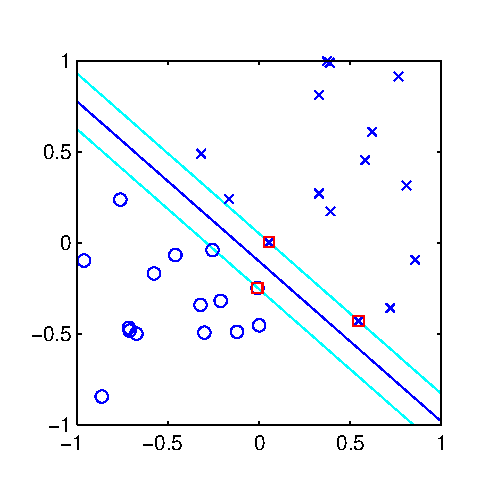
\includegraphics[width=1\textwidth]{1linesqp.eps}
          \caption{\label{Fig:ex1_1}line separated, SQP-like L-SVM}
        \end{minipage}
        \begin{minipage}[t]{0.24\linewidth}
          \centering
          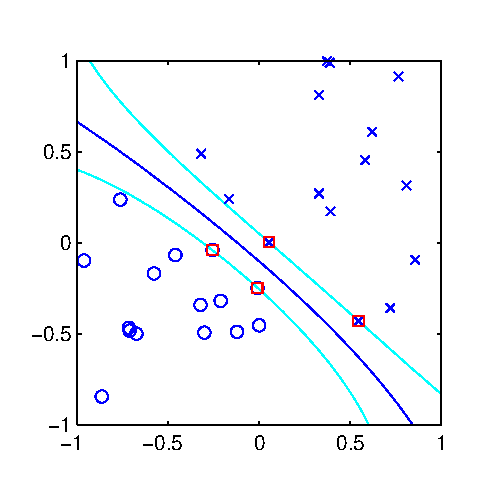
\includegraphics[width=1\textwidth]{1linechol.eps}
          \caption{\label{Fig:ex1_2}line separated, NL-SVM with fac.}
        \end{minipage}
        \begin{minipage}[t]{0.24\linewidth}
          \centering
          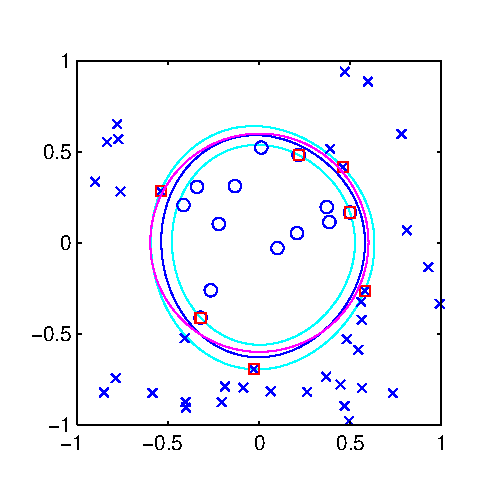
\includegraphics[width=1\textwidth]{1circlechol.eps}
          \caption{\label{Fig:ex1_3}circle separated, NL-SVM with fac.}
        \end{minipage}
        \begin{minipage}[t]{0.24\linewidth}
          \centering
          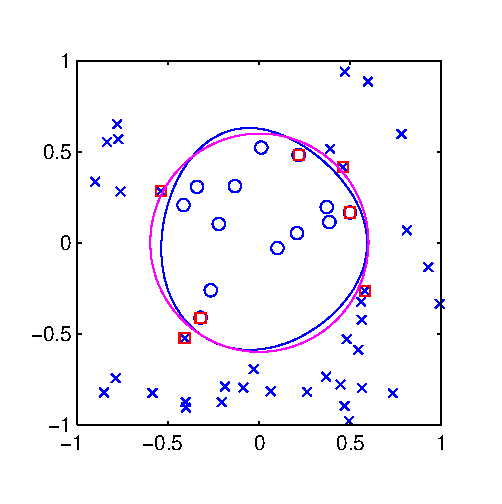
\includegraphics[width=1\textwidth]{1circlel1qp.eps}
          \caption{\label{Fig:ex1_4}circle separated, NL-SVM with L1QP.}
        \end{minipage}
      \end{figure}

      We begin with some very fundamental examples, where the distribution of data points follows basic patterns. Not only did these sets of experiments assist in the development of our codes, but they ideally enable us to depict some rudimental concepts visually as well.

      The simplest case is separable with a straight line, in which points lie in range $\left[-1,1\right]^{2}$ and on different sides of $x+y=0$. Figure \ref{Fig:ex1_1} shows how the SQP-like algorithm for the linear SVM model performs. As can be seen in the plot, the \textit{blue} diagonal line in the middle represents the OSH, alone with \textit{cyan} lines marking the distance of separation, \textit{i.e.} the $\pm h$ contour. We notice that due to absence of points from some corners, the OSH found shall be viewed as fairly good. Three supporting vectors are identified with \textit{red} square markers. In figure \ref{Fig:ex1_2}, the non-linear SVM based on full Cholesky factorization is also applied and, without doubt, separates the points as finely.

      In terms of non-linear separation, we visualize the example in section \ref{Sec:NLSVM} where the circle is centered at origin and has a radius of $0.6$ (drawn in pink). Figures \ref{Fig:ex1_3} and \ref{Fig:ex1_4} depict the resulting separation using factorization-based SVM and L1QP method\footnote{Due to limitations of the SVM package, we are currently unable to plot the $\pm h$ contours of L1QP.}, respectively. Since we have chosen the Gaussian kernel analogous to an exponential function, the separation attained is rather satisfactory and takes only a few supporting vectors.

      It is more worthy to point out that in the experiment, we observe that when $m\sim 100$, the built-in function \textsf{chol} for full Cholesky factorization often reports singularity of $K$. We conjecture that this happens because of ill-conditioning, which again justifies the use of partial decomposition.

    \subsection{Chessboards\label{Sec:Chess}}
      \begin{figure}[htbp]
        \centering
        \begin{minipage}[t]{0.24\linewidth}
          \centering
          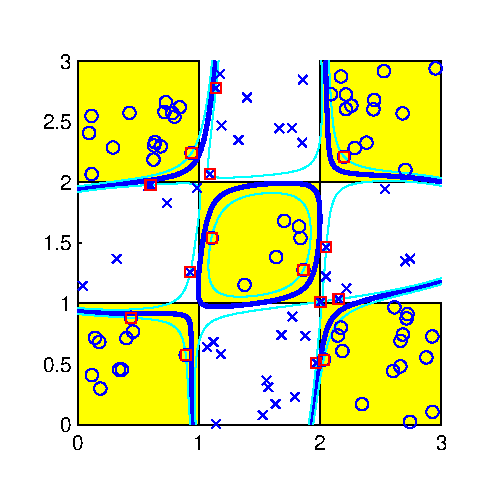
\includegraphics[width=1\textwidth]{2_3x3_chol.eps}
          \caption{\label{Fig:ex2_1}full chol. fac.}
        \end{minipage}
        \begin{minipage}[t]{0.24\linewidth}
          \centering
          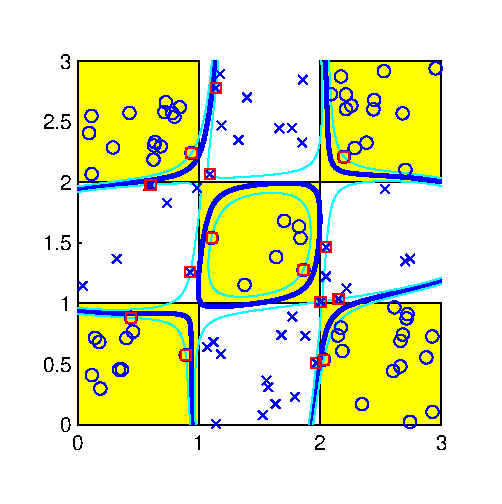
\includegraphics[width=1\textwidth]{2_3x3_pchol_1.eps}
          \caption{\label{Fig:ex2_2}\textsf{partchol}, w.\protect\\$\sigma=1,~tol=10^{-5}$}
        \end{minipage}
        \begin{minipage}[t]{0.24\linewidth}
          \centering
          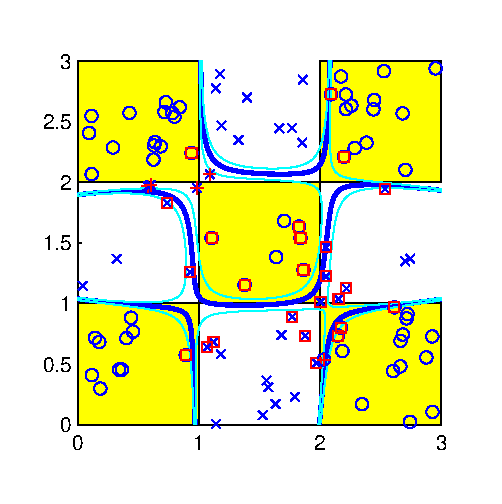
\includegraphics[width=1\textwidth]{2_3x3_pchol_sigma4.eps}
          \caption{\label{Fig:ex2_3}\textsf{partchol}, w.\protect\\$\sigma=4,~tol=10^{-5}$}
        \end{minipage}
        \begin{minipage}[t]{0.24\linewidth}
          \centering
          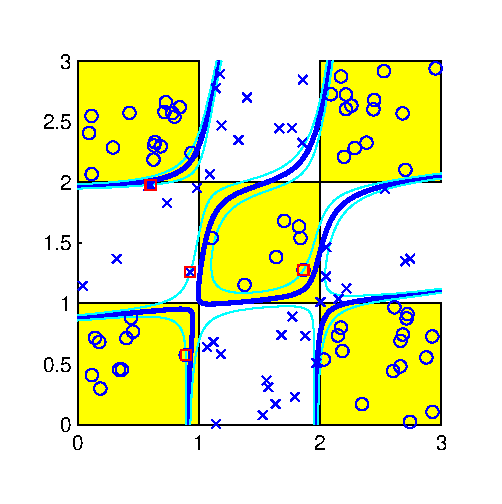
\includegraphics[width=1\textwidth]{2_3x3_pchol_tol10-2.eps}
          \caption{\label{Fig:ex2_4}\textsf{partchol}, w.\protect\\$\sigma=1,~tol=10^{-2}$}
        \end{minipage}
      \end{figure}
      To accord with the original work \cite{fletcher2010binary}, we have reproduced the chessboard sample problem to demonstrate some properties and comparison between the two methods.

      Figure \ref{Fig:ex2_1}, which is derived using full Cholesky decomposition and the SQP-like algorithm, shows a satisfying separation. While the absence of data points in some places might confuse the SVM, the blue contour matches considerably well with the squares. Precisely speaking, the SQP-like algorithm takes $9$ iterations to converge below $\tau_{d}=10^{-5}$ and $15$ support vectors are identified\footnote{It remains a minor problem for us how to reliably find support vectors when solving the primal and where there are truncation errors.}. In addition, to measure the \textit{generalization ability}, which means the efficiency in classifying \textit{unseen} points, a Monte-Carlo-like test is practiced. We evenly select $100\times 100$ points on the plane for classification, and this \textit{test error} in this case is merely $8.68\%$.

      The same data is used to train an SVM with \textsf{partchol}, and figure \ref{Fig:ex2_2} shows what it produces. After close inspection, it is still indistinguishable from figure \ref{Fig:ex2_1}. We notice that $\text{rank}(U)=45$ which halves the size of $K$ and it still produces 15 support vectors. The test error is $8.71\%$, proving that essentially no precision is compromised, if parameters are chosen properly.

      However, figures \ref{Fig:ex2_3} and \ref{Fig:ex2_4} suggest that this is not always the case. First, we modify the parameter $\sigma$ in the Gaussian kernel. It is discerned that when $\sigma$ seem to mismatch the magnitude of the average ``distance'' among data, strange behaviors tend to emerge. For instance, the test error becomes $9.48\%$ in figure \ref{Fig:ex2_3} where $\sigma=4$, and when $\sigma\geq 5$, the zero contours look like two circles. Yet the algorithms are not to blame since it is a kernel's issue. Second, if we enlarge $tol$ as in figure \ref{Fig:ex2_4}, leading to less approximation to $K$, the resulting classification may neither be as good. Conversely, too small a $tol$ brings about ``large'' and ill-conditioning $U$, which is also troublesome.

      Table \ref{Tab:ex2} lists numerical results in figures \ref{Fig:ex2_1}-\ref{Fig:ex2_4}, but more experiments were done in reality yet omitted in this report.
      % Table generated by Excel2LaTeX from sheet 'Sheet1'
        \begin{savenotes}\begin{table}[htbp]
          \centering
            \begin{tabular}{rrrr|rrrrr|r}
            \toprule
            fac.  & m       & $\sigma$ & $tol$     & rank$(U)$  & iter.   & \#SV    & miscl.\footnote{See below.} & err.      & fig. \\
            \midrule
            full  & $100$   & $1$      & $10^{-5}$ & n/a        & $9$     & $15$    & $0$     & $8.68\%$  & \ref{Fig:ex2_1} \\
            part  & $100$   & $1$      & $10^{-5}$ & $45$       & $8$     & $15$    & $0$     & $8.71\%$  & \ref{Fig:ex2_2} \\
            part  & $100$   & $4$      & $10^{-5}$ & $12$       & $2$     & $25$    & $5$     & $9.48\%$  & \ref{Fig:ex2_3} \\
            part  & $100$   & $1$      & $10^{-2}$ & $20$       & $8$     & $10$    & $0$     & $9.14\%$  & \ref{Fig:ex2_4} \\
            \bottomrule
            \end{tabular}%
          \caption{Results of the SVM with full/partial factorization on the $3\times 3$ chessboard problem.}
          \label{Tab:ex2}%
        \end{table}\end{savenotes}%

      \begin{figure}[htbp]
        \centering
        \begin{minipage}[t]{0.24\linewidth}
          \centering
          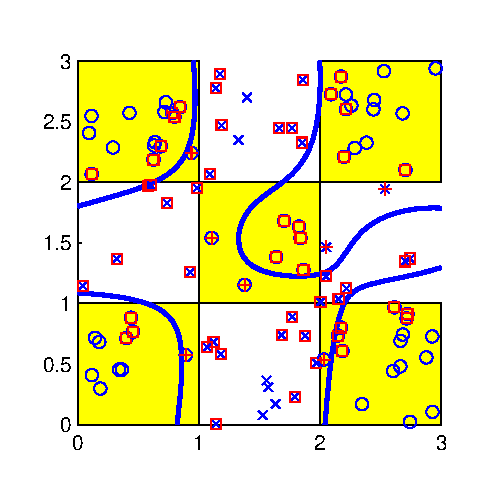
\includegraphics[width=1\textwidth]{2_3x3_l1qp_2.eps}
          \caption{\label{Fig:ex3_1}L1QP, $c=2$}
        \end{minipage}
        \begin{minipage}[t]{0.24\linewidth}
          \centering
          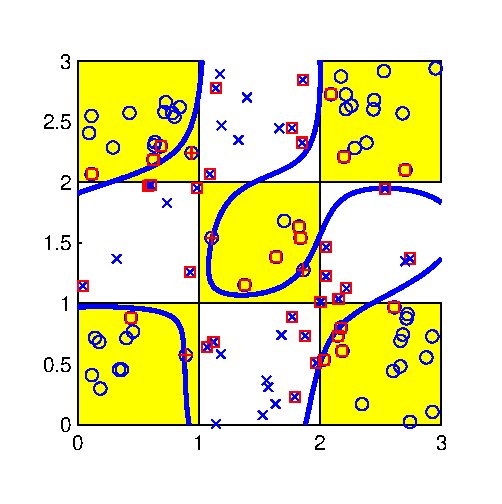
\includegraphics[width=1\textwidth]{2_3x3_l1qp_10.eps}
          \caption{\label{Fig:ex3_2}L1QP, $c=10$}
        \end{minipage}
        \begin{minipage}[t]{0.24\linewidth}
          \centering
          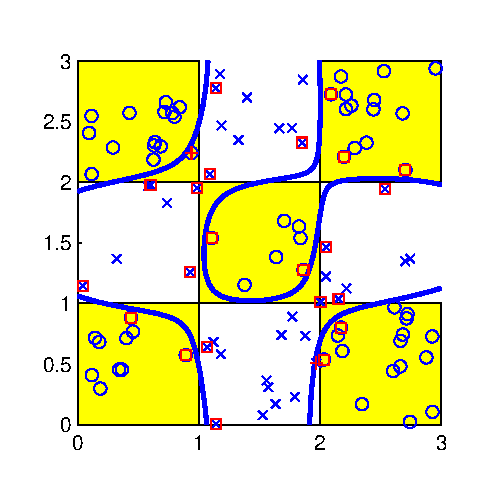
\includegraphics[width=1\textwidth]{2_3x3_l1qp_100.eps}
          \caption{\label{Fig:ex3_3}L1QP, $c=100$}
        \end{minipage}
        \begin{minipage}[t]{0.24\linewidth}
          \centering
          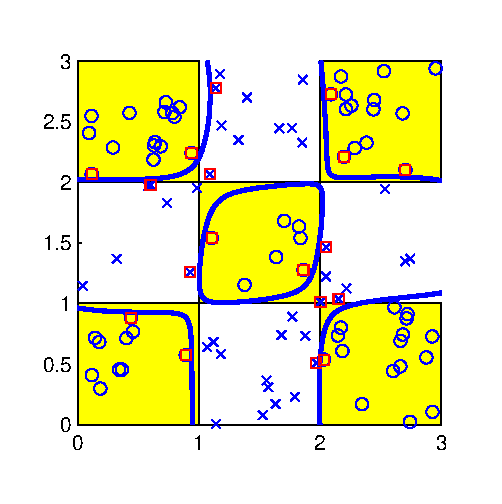
\includegraphics[width=1\textwidth]{2_3x3_l1qp_1000.eps}
          \caption{\label{Fig:ex3_4}L1QP, $c=10^{3}$}
        \end{minipage}
      \end{figure}
      Now we turn to analyzing the L1QP algorithm. As stated, the penalty $c$ deserves careful choice, which is perfectly illustrated in figures \ref{Fig:ex3_1}-\ref{Fig:ex3_4}.

      Data points lying on the wrong side of the zero contour, or the \textit{misclassified}, are marked with a cross. It can be seen in figure \ref{Fig:ex3_1} that too small a $c$ does not exert enough penalty on misclassifications and therefore encourages maximizing ``separation'' excessively. In fact, when $c\leq 1$ the zero contours make no sense at all. On the other hand, ``increasing $c$ gives fewer multipliers meeting their upper bound'' \cite{fletcher2010binary} (\textit{i.e.} fewer support vectors), so classification is more accurate. Eventually a good separation is attained when $c=1000$ (see figure \ref{Fig:ex3_4}). We summarize the numerical results in table \ref{Tab:ex3}.
      % Table generated by Excel2LaTeX from sheet 'Sheet1'
        \begin{savenotes}\begin{table}[htbp]
          \centering
            \begin{tabular}{r|rrr|r}
            \toprule
            $c$    & \#SV    & miscl.  & err.      & fig. \\
            \midrule
            $2$    & $59$    & $7$     & $19.55\%$ & \ref{Fig:ex3_1} \\
            $10$   & $39$    & $4$     & $12.66\%$ & \ref{Fig:ex3_2} \\
            $100$  & $22$    & $2$     & $8.71\%$  & \ref{Fig:ex3_3} \\
            $1000$ & $18$    & $0$     & $8.25\%$  & \ref{Fig:ex3_4} \\
            \bottomrule
            \end{tabular}%
          \caption{Results of the SVM with L1QP on the $3\times 3$ chessboard problem. In all settings, $m=100,~\sigma=1$.}
          \label{Tab:ex3}%
        \end{table}\end{savenotes}%

      \begin{savenotes}\begin{figure}[htbp]
        \centering
        \begin{minipage}[t]{0.48\linewidth}
          \centering
          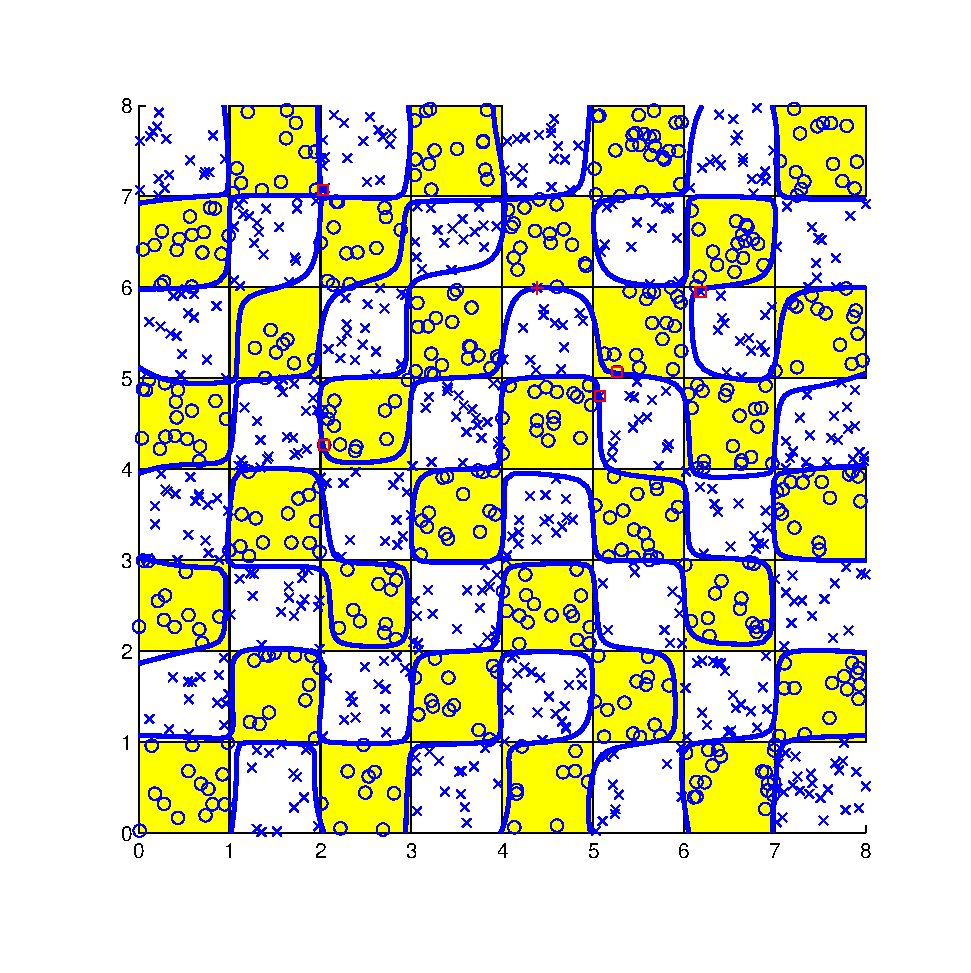
\includegraphics[width=1\textwidth]{2_8x8_1000.eps}
          \caption{\label{Fig:ex4_1}\textsf{partchol} with $1000$ samples}
        \end{minipage}
        \begin{minipage}[t]{0.48\linewidth}
          \centering
          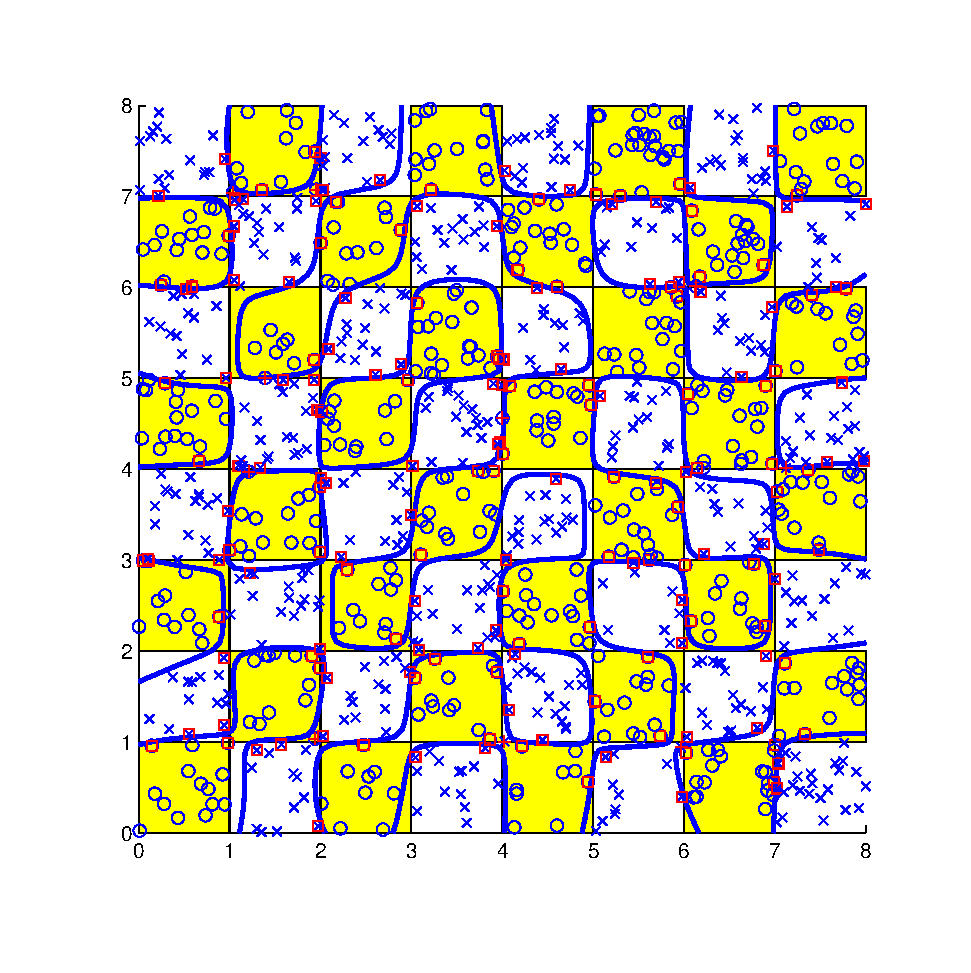
\includegraphics[width=1\textwidth]{2_8x8_1000_l1qp.eps}
          \caption{\label{Fig:ex4_2}L1QP with the same data set}
        \end{minipage}
      \end{figure}\end{savenotes}

      Next to investigate is how well \textsf{solve\_nlp\_pchol} deals with larger amounts of (training) data. A much larger $8\times 8$ chessboard is utilized and the number of points $m$ increases to $1000$. The parameters are still $\sigma=1,~\tau_{d}=10^{-5},~tol=10^{-5}$. The resulting separation is visualized\footnote{Not all support vectors are marked.} in figure \ref{Fig:ex4_1}. Numerically, we observe $\text{rank}(U)=213$, with approximately $21$ iterations required for the SQP-like algorithm, and the test error is $10.45\%$. Since we did not intend to perform tests with respect to various parameters, and $m$ is not too large compared to the number of squares, this is a fairly desirable outcome. Figure \ref{Fig:ex4_2} shows tests of the L1QP method for comparison. Its test error is $8.92\%$.

      It occurred to the authors, at the time of composing this report, that the tolerance of the QP solver \textsf{quadprog} is also of some significance. In Fletcher's paper \cite{fletcher2010binary}, for instance, his own \textsf{BQPD} code is adopted. We plan to address this aspect in the future.

    \subsection{MNIST Handwritten Numbers\label{Sec:MNIST}}
      Some preliminary tests have also been done with \textit{The MNIST database of handwritten digits} \cite{lecun1998mnist}. This is a set of $28\times 28$ pixels grey-scale images of digits $0$ to $9$ written by different people. Since our SVMs are binary classifiers, we simplify the task to distinguishing $1$'s from $9$'s.

      We pick $m=400$ images from \emph{each} category, and an additional $t=160$ \emph{unseen} images to test generalization. As recommended \cite{fletcher2010binary}, let $\sigma=1800$ (since the vectors have $28\times 28=784$ dimensions) and $tol=10^{-3}$. It is observed that matrix $U$ has $312$ rows, SQP takes $12$ iterations to converge, no misclassification happens and test error is only $1/160$. If $\sigma$ equals $100$ and $50000$, the test error becomes $100\%$ and $12.5\%$, respectively.

      Since our implements of these SVM variants are for demonstrational purposes, we defer tests on other large-scale data sets. To apply our binary separating SVMs to multi-class classification problems, many different approaches have been developed. See \cite{hsu2002comparison,duan2005best} for detail.

    \subsection{Mislabel and Improvements\label{Sec:Issues}}
      What if some samples are \textit{mislabelled} in the training set? This is actually ubiquitous in real-world problems. For example, in most visual object databases (\textit{e.g.} PASCAL VOC \cite{everingham2010pascal} and ImageNet \cite{deng2009imagenet}) classification was done by humans, so errors are inevitable. However, we will see that the SQP-like algorithm at this stage tends to struggle in order to get perfect separation, which in turn brings about strange behaviors and reduces generalization abilities.

      \begin{figure}[htbp]
        \centering
        \begin{minipage}[t]{0.31\linewidth}
          \centering
          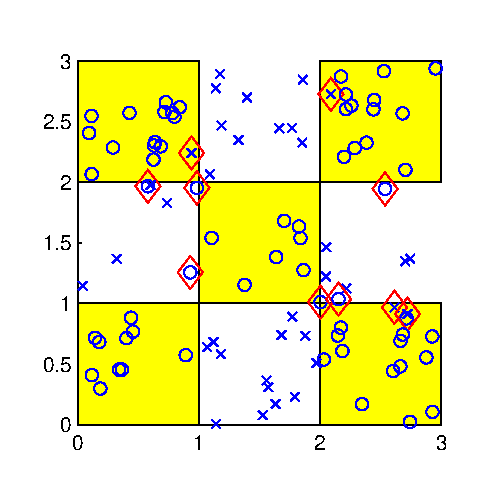
\includegraphics[width=1\textwidth]{4_3x3_mislabel.eps}
          \caption{\label{Fig:ex5_1}$10$ points are intentionally mislabelled}
        \end{minipage}
        \begin{minipage}[t]{0.31\linewidth}
          \centering
          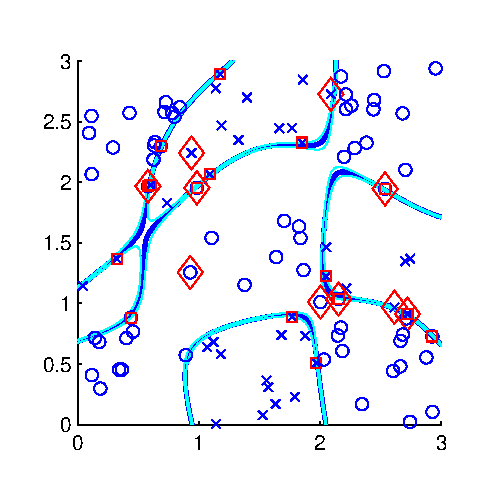
\includegraphics[width=1\textwidth]{4_3x3_mislabel_pchol.eps}
          \caption{\label{Fig:ex5_2}\textsf{partchol} solution}
        \end{minipage}
        \begin{minipage}[t]{0.31\linewidth}
          \centering
          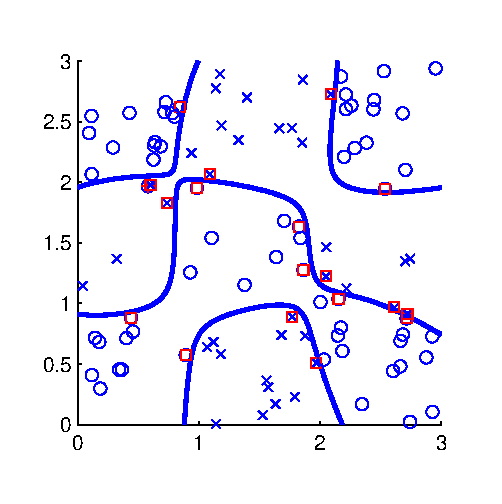
\includegraphics[width=1\textwidth]{4_3x3_mislabel_l1qp.eps}
          \caption{\label{Fig:ex5_3}L1QP solution with $c=1000$}
        \end{minipage}
      \end{figure}
      Some $10$ points near the border lines have had their labels intentionally inverted and are marked with red diamonds in figure \ref{Fig:ex5_1}. This simulates mislabeling due to observation errors. With the same parameters as in figure \ref{Fig:ex2_2}, \textsf{partchol} now produces less satisfactory contours in figure \ref{Fig:ex5_2}. Despite its efforts to avoid any misclassification, the curve itself gets rather distorted and separation ($h_{*}$) is marginal, since the cyan $\pm h$ contours overlay with the blue zero contours. The test error soars towards $21.20\%$. In comparison, we deployed the L1QP-SVM as in figure \ref{Fig:ex3_4}. The results in figure \ref{Fig:ex5_3} appear to be relatively better with $12.34\%$ test error. Only a couple of misclassifications occur as a token to pay, and it could possibly be further tuned with different choices of $c$.

      As a remedy, Fletcher et al. \cite{fletcher2010binary} have suggested an auxiliary problem to SP. When too small an $h_{*}$ is detected, signifying poor separation (with possibly too many support vectors), they propose a \textit{desired margin} $\hat{h}>h_{*}$ and an $\mathcal{L}_{1}$ slack variable $\vec{\xi}$. They then derive the following NLP problem
      \begin{align}
        \mathop{\text{minimize}}_{\vec{w},b,\vec{\xi}}~~ & \vec{e}^{\mathrm{T}}\vec{\xi} \label{Eqn:SPrelax1}\\
        \text{subject to}~~ & AV^{\mathrm{T}}\vec{w}+\vec{a}b+\vec{\xi}\geq\vec{e}\hat{h}, \label{Eqn:SPrelax2}\\
        & \vec{w}^{\mathrm{T}}\vec{w}=1, \label{Eqn:SPrelax3}\\
        \text{and}~~ & \vec{\xi}\geq\vec{0}, \label{Eqn:SPrelax4}
      \end{align}
      which is the most elegant solution we can currently devise.

  \section{Conclusion\label{Sec:FIN}}
    In this report, we give a close examination over the problem of binary separation with support vector machines. The standard formulation of separation in linearly separable, non-separable, and non-linearly separating settings are derived. Once exact separation is not possible or not preferable, the problem instant becomes a non-convex quadratic programming which is difficult to solve. The traditional approach introduces the use of $\mathcal{L}_{1}$-penalties and relies on its dual problem to construct a convex QP, also known as the L1QP method. However, this treatment has incurred some issues, and direct solution of the primal draws the interest of many. We describe an SQP-like algorithm proposed by Fletcher et al. \cite{fletcher2010binary} that facilitates the attainment of solution. For non-linear problems, kernel functions are used to readily reduce it to a previous one. It can be naturally incorporated into dual-based methods without difficulties, but primal ones require further consideration. For this purpose, (partial) Cholesky factorization is utilized and some work \cite{fletcher2010binary} focus on further improving computational costs and conditioning.

    After these detailed description, we implement the two approaches in \textsf{MATLAB} to examine their performance through a series of experiments. While the chessboard and MNIST problem both demonstrate that the SQP-NLSVM with \textsf{partchol} often outperform L1QP, it is noticed that in the presence of mislabelled samples, the former may run into difficulties. The reason of this phenomenon is tentatively analysed, and we present the recommendations of Fletcher et al. \cite{fletcher2010binary} for remedy.

    What distinguishes this reading report is the detailed rationale and proof added to the original paper, in addition to some valuable insights from the authors' own experience. It is our hope that the Tsinghua student have by now grasped the rudimental theory of SVM in this report.

  \bibliographystyle{plain}
  \bibliography{bibtex}
\end{document}
